% 1977 年辽宁卷第五题证法一：梯形 ABCD（DC∥AB），CE⊥AB 于 E、DF⊥AB 于 F（按源卷第 3 页「第五题证法一附图」布局）
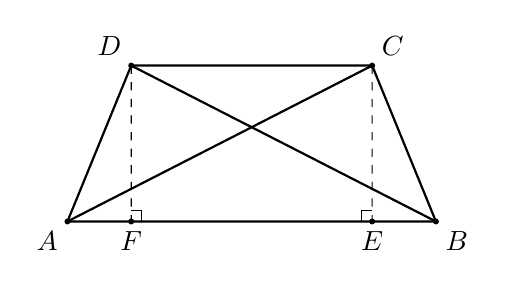
\begin{tikzpicture}[scale=0.9]
  \coordinate (A) at (0,0);
  \coordinate (B) at (5.2,0);
  \coordinate (D) at (0.9,2.2);
  \coordinate (C) at (4.3,2.2);
  \draw[thick] (A)--(B)--(C)--(D)--cycle;
  \draw[thick] (A)--(C);
  \draw[thick] (B)--(D);
  \draw[dashed] (C)--(4.3,0);
  \draw[dashed] (D)--(0.9,0);
  \fill (A) circle (1.2pt) node[below left] {$A$};
  \fill (B) circle (1.2pt) node[below right] {$B$};
  \fill (D) circle (1.2pt) node[above left] {$D$};
  \fill (C) circle (1.2pt) node[above right] {$C$};
  \fill (4.3,0) circle (1.2pt) node[below] {$E$};
  \fill (0.9,0) circle (1.2pt) node[below] {$F$};
  % 直角标记
  \draw[thin] (4.15,0) -- (4.15,0.15) -- (4.3,0.15);
  \draw[thin] (1.05,0) -- (1.05,0.15) -- (0.9,0.15);
\end{tikzpicture}
